
\documentclass[a4paper, 10pt]{IEEEconf}  

\usepackage{geometry}
\geometry{a4paper, margin=1in}
  
  
\usepackage{subcaption}  
\usepackage[export]{adjustbox}    
\usepackage{verbatim}
\usepackage{graphicx}
\usepackage{pdfpages}
\usepackage{cite}
\usepackage{listings}
\usepackage{float}
\usepackage{url}
\usepackage{hyperref}
\usepackage{fancyhdr}
\usepackage{multicol}

\lstset{
	tabsize=2,
	breaklines=true
}

\setlength{\parskip}{1em}
\onecolumn

\title{\LARGE \bf Assignment 4: Vision-based Automatic Systems\\Industrial Systems Design and Integration 282 772}
\author{Marc Alexander Sferrazza \\ 12164165
\thanks{This work was not supported by any organization}
\thanks{Faculty of Mechatronics Engineering, Massey University, Albany, Auckland, New Zealand
        {\tt\small Progress of project: https://github.com/alex1v1a/Industrial-Systems-Design-and-Integration} } }

\begin{document}

\maketitle
\begin{figure}[H]
  \begin{center}
  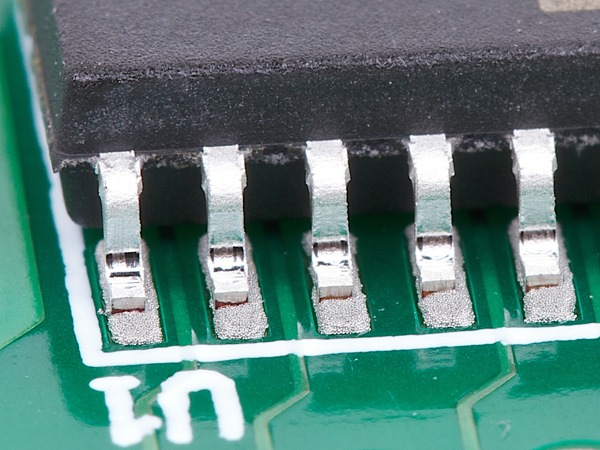
\includegraphics[width=110mm]{images/match}
  \label{fig:kinetic}
  \end{center}
\end{figure}
\thispagestyle{empty}
\pagestyle{plain}


%%%%%%%%%%%%%%%%%%%%%%%%%%%%%%%%%%%%%%%%%%%%%%%%%%%%%%%%%%%%%%%%%%%%%%%%%%%%%%%%

\begin{abstract}
In this assessment, you are to design a system that can pick and place electronic Surface Mount Device (SMD) components onto a Printed Circuit Board (PCB) and validates their correct alignment using vision.

%In this documentation TensorFlow's neural network machine learning is used to find a function for y=f(x) given some inputs and outputs. The process involves using the Multi-Layered Perceptron (MLP) technique training and placeholders are used to provide input.
\end{abstract}


 

%%%%%%%%%%%%%%%%%%%%%%%%%%%%%%%%%%%%%%%%%%%%%%%%%%%%%%%%%%%%%%%%%%%%%%%%%%%%%%%%
%%%%%%%%%%%%%%%%%%%%%%%%%%%%%%%%%%%%%%%%%%%%%%%%%%%%%%%%%%%%%%%%%%%%%%%%%%%%%%%%
\clearpage
\setcounter{page}{1}
%\thispagestyle{empty}
\onecolumn

\section{INTRODUCTION}

In this assessment, you are to design a system that can pick and place electronic Surface Mount Device (SMD) components onto a Printed Circuit Board (PCB) and validates their correct alignment using vision.

%TensorFlow is a free(open-source) python language based library which is used for machine learning (intelligence) using neural networks to determine functions based on given inputs and outputs\cite{ML}. As TensorFlow (TF) is supported by the community it makes as a favourable tool to learn, and is not only capable of black box systems, but also able to coordinate with complex systems with learning nodes.
%
%In this documentation the program TensorFlow is used to train a neural network that will approximate an unknown function of y=f(x) for a given vector. Using Python 3.5+ syntax and TensorFlow 1.0+ syntax, a predefined data set csv file will be called on which to preform the learning task for an output range.


%%%%%%%%%%%%%%%%%%%%%%%%%%%%%%%%%%%%%%%%%%%%%%%%%%%%%%%%%%%%%%%%%%%%%%%%%%%%%%%%

\subsection{Aim}

Apply the principles and technologies in intelligent machine design and integration.
Demonstrate familiarity with industrial vision systems and vision-based automatic systems.


\begin{figure}[H]
  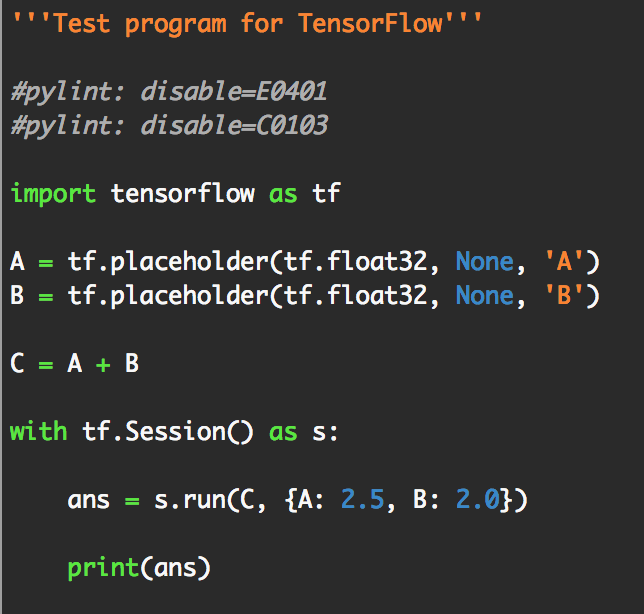
\includegraphics[width=0.5\linewidth,center]{images/test}
  \caption{lalalala}
  \label{fig:lalalala}
\end{figure}

%%%%%%%%%%%%%%%%%%%%%%%%%%%%%%%%%%%%%%%%%%%%%%%%%%%%%%%%%%%%%%%%%%%%%%%%%%%%%%%%
%%%%%%%%%%%%%%%%%%%%%%%%%%%%%%%%%%%%%%%%%%%%%%%%%%%%%%%%%%%%%%%%%%%%%%%%%%%%%%%%
%\clearpage
\section{Environment}
%0.5pg 


%%%%%%%%%%%%%%%%%%%%%%%%%%%%%%%%%%%%%%%%%%%%%%%%%%%%%%%%%%%%%%%%%%%%%%%%%%%%%%%%
%\clearpage
\subsection{Concepts}

Several concepts are presented and evaluated using an appropriate quantitative assessment.

%%%%%%%%%%%%%%%%%%%%%%%%%%%%%%%%%%%%%%%%%%%%%%%%%%%%%%%%%%%%%%%%%%%%%%%%%%%%%%%%
%%%%%%%%%%%%%%%%%%%%%%%%%%%%%%%%%%%%%%%%%%%%%%%%%%%%%%%%%%%%%%%%%%%%%%%%%%%%%%%%
%\clearpage
\section{CONSTRAINTS} 
%0.5pg

%%%%%%%%%%%%%%%%%%%%%%%%%%%%%%%%%%%%%%%%%%%%%%%%%%%%%%%%%%%%%%%%%%%%%%%%%%%%%%%%

\subsection{Developments}

Several developments are presented and changes de- scribed and discussed, and evaluated using an appropriate quantitative assessment.

%%%%%%%%%%%%%%%%%%%%%%%%%%%%%%%%%%%%%%%%%%%%%%%%%%%%%%%%%%%%%%%%%%%%%%%%%%%%%%%%
%\clearpage
\subsection{Evaluations}

%%%%%%%%%%%%%%%%%%%%%%%%%%%%%%%%%%%%%%%%%%%%%%%%%%%%%%%%%%%%%%%%%%%%%%%%%%%%%%%%
%\clearpage
\subsection{Final Design}

A final design is presented and described and discussed in detail.

%%%%%%%%%%%%%%%%%%%%%%%%%%%%%%%%%%%%%%%%%%%%%%%%%%%%%%%%%%%%%%%%%%%%%%%%%%%%%%%%
%%%%%%%%%%%%%%%%%%%%%%%%%%%%%%%%%%%%%%%%%%%%%%%%%%%%%%%%%%%%%%%%%%%%%%%%%%%%%%%%

\section{CRITIQUE}
%1pg

%%%%%%%%%%%%%%%%%%%%%%%%%%%%%%%%%%%%%%%%%%%%%%%%%%%%%%%%%%%%%%%%%%%%%%%%%%%%%%%%
%\clearpage
\subsection{Machine-vision Algorithm}

A machine vision algorithm is described and discussed in detail.

%%%%%%%%%%%%%%%%%%%%%%%%%%%%%%%%%%%%%%%%%%%%%%%%%%%%%%%%%%%%%%%%%%%%%%%%%%%%%%%%
%%%%%%%%%%%%%%%%%%%%%%%%%%%%%%%%%%%%%%%%%%%%%%%%%%%%%%%%%%%%%%%%%%%%%%%%%%%%%%%%

\section{SOLUTIONS}
%1pg

short description of the machines operation.


critical reflection of your design process.

A detailed critical reflection of the employed design process is presented.

%The machine learning task was completed with best results using MLP and the Adam Optimisation technique. The node size is optimal from 20+ with a learning rate less then 0.02 and epochy (iterations) are subjectible.

%%%%%%%%%%%%%%%%%%%%%%%%%%%%%%%%%%%%%%%%%%%%%%%%%%%%%%%%%%%%%%%%%%%%%%%%%%%%%%%%
%%%%%%%%%%%%%%%%%%%%%%%%%%%%%%%%%%%%%%%%%%%%%%%%%%%%%%%%%%%%%%%%%%%%%%%%%%%%%%%%

\section{CONCLUSIONS}

%For any progress related to the report please see the public Github repo for alex1v1a or use the link in the cover page to be automatically redirected to this project. The repo provides all relative project information
%
%I have come to a further understanding learned the fundamentals of TensorFlow's with nodes and tensors, and the use of such machine learning tools like Multi-Layered Perceptron using placeholders. This is a powerful tool and from a basic level of understanding is a strong aspect of machine learning processing, it is a great skill to learn. 
%
%The appendix contains a full documentation of my modified version of Frazer Nobles GitHub Tutorial 4 - Unfortunately I was unable to use Tutorial 6 to complete this assignment after several attempts using Batching.

%%%%%%%%%%%%%%%%%%%%%%%%%%%%%%%%%%%%%%%%%%%%%%%%%%%%%%%%%%%%%%%%%%%%%%%%%%%%%%%%
%%%%%%%%%%%%%%%%%%%%%%%%%%%%%%%%%%%%%%%%%%%%%%%%%%%%%%%%%%%%%%%%%%%%%%%%%%%%%%%%

\nocite{*}
\bibliographystyle{ieeetr}
\bibliography{references}

%%%%%%%%%%%%%%%%%%%%%%%%%%%%%%%%%%%%%%%%%%%%%%%%%%%%%%%%%%%%%%%%%%%%%%%%%%%%%%%%
%%%%%%%%%%%%%%%%%%%%%%%%%%%%%%%%%%%%%%%%%%%%%%%%%%%%%%%%%%%%%%%%%%%%%%%%%%%%%%%%

%\clearpage
%\onecolumn
%\section*{APPENDIX}
%\begin{lstlisting}[language = Python]
%\end{lstlisting}

\end{document}
